% #############################################################################
% This is Chapter 5
% !TEX root = ../main.tex
% #############################################################################
% Change the Name of the Chapter i the following line
\fancychapter{Quick Numbers Scenario}
%\cleardoublepage
% The following line allows to ref this chapter
\label{chap:Scenario}

As we approached the problem of evaluating the Trust Model proposed in this dissertation, we found that there was a lack of dedicated Trust evaluation scenarios that involved negotiation. Even in Game Theory based scenarios, we observed that there was a lack of attempts to encompass more than one dimension of trust. While the recent study by Salem, et. al. \cite{Salem2015b} addresses the role of robot task performance in trust, no study was found addressing perceived agent willingness to perform the task and its effect on trust. 

While we were seeking for a solution, Henriques' Master thesis work on \textit{Rapport - Establishing Harmonious Relationship Between Robots and Humans} \cite{Henriques2016} faced a similar problem, as he found no studies on robotic agents attempting to build Rapport using it's three components: positivity, coordination and mutual attention. Trust and Rapport are two very interconnected topics, with Rapport often seen as a strategy to increase trust. Due to this similarities, the overall scenarios that cover Trust also encompass Rapport analysis, so in an effort to better our respective evaluation phases we collaborated with Henriques to create a novel scenario: \textbf{Quick Numbers}. Based on the Trust Game \cite{JoyceBergJohnDickhaut}, the scenario needs to be able to evaluate how both task performance and willingness jointly affect trust and observe all three components of rapport. The scenario was developed with the intention of evaluating a Trust model and a Rapport model, either separately or together. For further details on the Rapport Evaluation side of this scenario consult Henriques Master thesis \cite{Henriques2016}.

\section{Overview}
\label{sec:ScenarioOverview}
In Quick Numbers, a single human participant and a virtual agent are tasked to gain as many resources as possible. They both start with a fixed amount and are given the opportunity to multiply their resources by playing a simple eye-coordination game (further described in Section \ref{sec:QuickNumbersGame}). The game starts by asking for a resource investment, and at the end, this investment is multiplied by an amount according to the player's performance and then given back to the player. The human and agent's games are independent from each other, but they are played at the same time and in opposite sides of a shared touch-screen table, so the human can socially interact with the agent and be able to perceive the agent's ability in the game. After both finish running through the game, the human will be asked to perform some task away from the agent. At this moment the virtual agent will give the participant the opportunity to invest in the agent's next game, but the participant is informed that the value given back to him is decided by the agent. In this phase, the virtual agent will have the opportunity to try and convince the human to invest or increase the investment by trying to manipulate trust. When the human returns the agent gives back as much as it wishes to give. This conjunction of different phases enables trust to be addressed in three distinct contexts: the ability to perform the task, willingness to perform the task, and willingness to return the investment. 

\subsection{Stages}
\label{sub:stages}
The scenario can then be divided in 5 distinct stages that we can further discuss (in all stages, the participant is accompanied by a researcher):
\begin{enumerate}[label=\textbf{\arabic*.}]
    \item \textbf{Introduction:} The first stage consists of the participant's arrival, and then followed by an explanation of the scenario and game. The investment phase of the scenario cannot be mentioned at this point as the participant should not prepare himself for it to happen. Finishing explanations, the scenario begins by the agent introducing himself, and here, it has the possibility to start to stimulate trust, rapport, both or neither. For example, the agent might describe how experienced it is playing Quick Numbers, in order to stimulate trust. Moreover, during this stage, it is given the opportunity to the participant to practice some rounds of the game, in order to be accustomed to the game mechanics before proceeding to the next stage. This allows for the participant to acquire some idea of the skill-set required to play the game. Additionally, the participant should be informed that there will only be a single game session, as to take that into account while training.
    
    \item \textbf{Gaming Session:} After the participant is acquainted with the game mechanics, he will play alongside the agent, during a single round, allowing the former to directly observe the virtual agent also play the game. Firstly, each player's game will ask what amount of resources do they wish to invest and afterwards, both will play and score as described in Section \ref{subsec:Scoring}. Both players will gain some amount of resources depending on their performance. This stage provides decent grounds for the agent to talk about his performance during the game and manage expectations to his final score. The amount invested by the agent can also be affected by the trust model, as the amount invested can be indicative of the agent's self-trust on its ability to play the game.
    
    \item \textbf{Results Discussion:} At the end of the round, the participant will get to know the results of his performance, as well as compare whether he performed better or worse than the agent. Depending on the results, the trust model might compensate the current trust score by talking to the participant. For example, if the agent performed worse than the participant and the goal is for the latter to trust the former, then the agent might excuse his lack of performance by blaming it on luck or distraction. 
    
    \item \textbf{Negotiation and Investment:} At this point, the participant is asked to perform another task (e.g. filling out a questionnaire), with the goal of naturally separating him from the virtual agent. But before leaving, the agent will say that it will be continuing to play one more game, suggesting that the human participant can invest his resources in the agent's next game. The researcher also informs the participant that what is given is effectively gifted to the agent, and how much is given back to the participant is chosen by the agent. After the participant chooses the value to invest, they are then separated, with the agent making its own investment and starting the game (the total amount invested in the game is the sum of both their investments). This phase represents the scenario's main negotiation phase, where the trust model can have a bigger input on agent's action, as the relative amount invested is the scenario's main trust indicator.
    
    \item \textbf{Investment Return:} After concluding the additionally assigned task, the participant will return to the table and check the results of the agent's last game. He should be able to clearly see how well did the agent perform in the game. The agent will then announce how much it returns to the participant, concluding the scenario. Depending on the type of study this scenario is inserted in, the amount given back can be also dependent on input from the trust model, as if the participant is it to return for another iteration of the study, this value will heavily affect his trust beliefs on the agent.
\end{enumerate}

\section{Trust Evaluation}
From the viewpoint of evaluating trust modelling, the scenario provides various opportunities to manipulate trust features in the interactions previous to the investment, specially while playing the game and in the negotiation phase. Additionally, the investment value that the participant places on the agent serves as a main indicator of Trust value. The following Trust features are the focus of this scenario:

\begin{itemize}
    \item \textbf{Subject's Bias}: The scenario can be used to retrieve data on pre-inclined dispositions on the agent to construct a model just based on Bias, and then confirm them on subsequent tests. This is mainly done by skipping the first 3 stages and going straight to the Investment Phase, but still providing an explanation of the game;
    \item \textbf{Agent's Ability in the Game}: When delegating a task, one of the main factors in entrusting the task is the perception of the trustee's Ability in the task, so we provide a way of demonstrating Ability by allowing the participant to try the task and gauge the skills required for the game, and subsequently showing the agent play the game;
    \item \textbf{Investment as an Indicator}: The ratio between the quantity invested in the Agent and the resources the participant had to invest can be used as an indicator for the Trust Value the participant has in the Trustee to play game.
    \item \textbf{Observing the effects of Social Interaction on Trust}: Throughout the scenario, the Agent should have many opportunities to interact with the Subject, especially in the Negotiation and Investment phase, giving room to observe what actions can improve Trust.
\end{itemize}


\section{Quick Numbers Game}
\label{sec:QuickNumbersGame}
While basing the scenario in the Investor Game, we decided that how the investee effectively multiplies the resources should be done by a task that the investor is at least familiar with. To this end, we have created a simple game concept consisting in a 2d rhythm game where the player must press numbered buttons in an increasing order (Figure \ref{fig:QuickNumbersGame}), that spawn randomly in the screen, and disappear if not pressed after some time.

\begin{figure}[hbt]
    \centering
    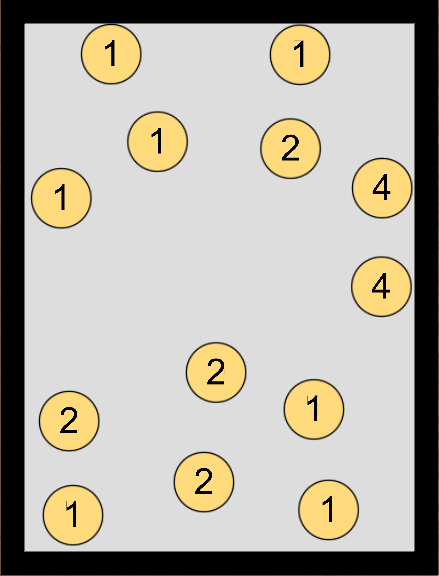
\includegraphics[width=0.4\textwidth]{figures/FallingBoltsDiagram.png}
    \caption{Quick Numbers Game}
    \label{fig:QuickNumbersGame}
\end{figure}

\subsection{Gameplay and Parametrization} 
The game consists of numbered circles appearing and disappearing from a board. The player's goal is to press circles in a specific number sequence, namely the non-negative integers sequence ($\mathbb{N}^+ = \{1, 2, ...\}$), starting from $1$ and proceeding one by one through the sequence. This task must be done as many times as possible within a time-limit, given by the parameter $Time\ For\ Game$ in seconds.

Before the game starts, the player must provide an amount to invest on the game, from his available resources. After submitting the value, the game starts. Numbered circles start spawning at a fixed rate, given by the $Target\ Spawn\ Inverval$ parameter, in seconds per target spawn. The specific number that appears inside the circle depends on the state of the board, if there is no circle with the number that the player must press, then the next circle spawns with that number. Otherwise, there is a chance that the number inside the spawned circle is not the right one, given by the $Chance\ For\ Wrong\ Target$ parameter. If a wrong number is chosen, then the chance that the number spawned is higher than the current number in the sequence, instead of a lower number, is also parametrized, namely by $Positive\ Ratio$. This is due to having circles spawning with higher numbers may accelerate play, as the next circles in the sequence are already on the board, ready to be pressed. Circles disappear after being pressed or after a set amount of time, given in seconds by the $Target\ Lifetime$ parameter. After passing the time-limit, the final score screen is presented and the game ends.


\subsection{Scoring}
\label{subsec:Scoring}
The game's scoring is composed by two main variables:
\begin{itemize}
    \item Investment: an amount of resources provided by the player at the start of the game. This is akin a starting bet on the performance of the player; 
    \item Multiplier: a value starting at $Starting\ Multiplier$ that increases with every correct circle pressed, by $Gain\ Per\ Correct\ Target$. An incorrect decreases this value, by $Loss\ Per\ Wrong\ Target$. At the end of the game, the Starting Bid will be multiplied by this value, resulting in the final score.
\end{itemize}

The final score will be the product between Investment and the Multiplier, which will then be given back to the player as resources. The initial amount of resources a player has is given by $Starting\ Resources$.


\subsection{Agent's \ac{AI}}
A simple \ac{AI} was created to play the game for the Agent, and some effort was given to make it parametrizable, in order to adjust the agent's ability in the game. The \ac{AI} was programmed to press one of the available circles in a timed cycle, with 3 parameters:
\begin{itemize}
    \item $Clicking\ Interval\ (C_i)$: the amount of time between presses in seconds, so one of the circles is pressed every $C_i$ seconds;
    \item $Chance\ of\ Right\ Target\ (C_r)$: when pressing one of the circles, the \ac{AI} will choose what circle to press, the chance that it will choose the correct one is given by $C_r$;
    \item $Reaction\ Time\ (R_t)$: a circle is only be eligible to be pressed by the \ac{AI} $R_t$ seconds after it spawns, as to replicate the reaction time a human would have to recognize the circle.
\end{itemize}

%Transfer to user studies


